Die Abbildung \ref{fig:diagrammInitial_worp} zeigt grafisch die Ergebnisse der
Messreihen für den initialen Durchlauf ohne Relevante Bereiche. Dabei ist die
Laufzeit in $µs$ über die Textgröße in Byte logarithmisch aufgetragen. Für
relativ kleine Textgrößen kommt die Geschwindigkeitsoptimierung noch nicht zum
Tragen. Erst bei einer Größe von $5.000.000$ ($99$ µs) oder $10.000.000$ ($122$
µs) Byte ist der erwartete Geschwindigkeitsprofit zu verzeichnen. 

\begin{figure}[H]
	\centering
	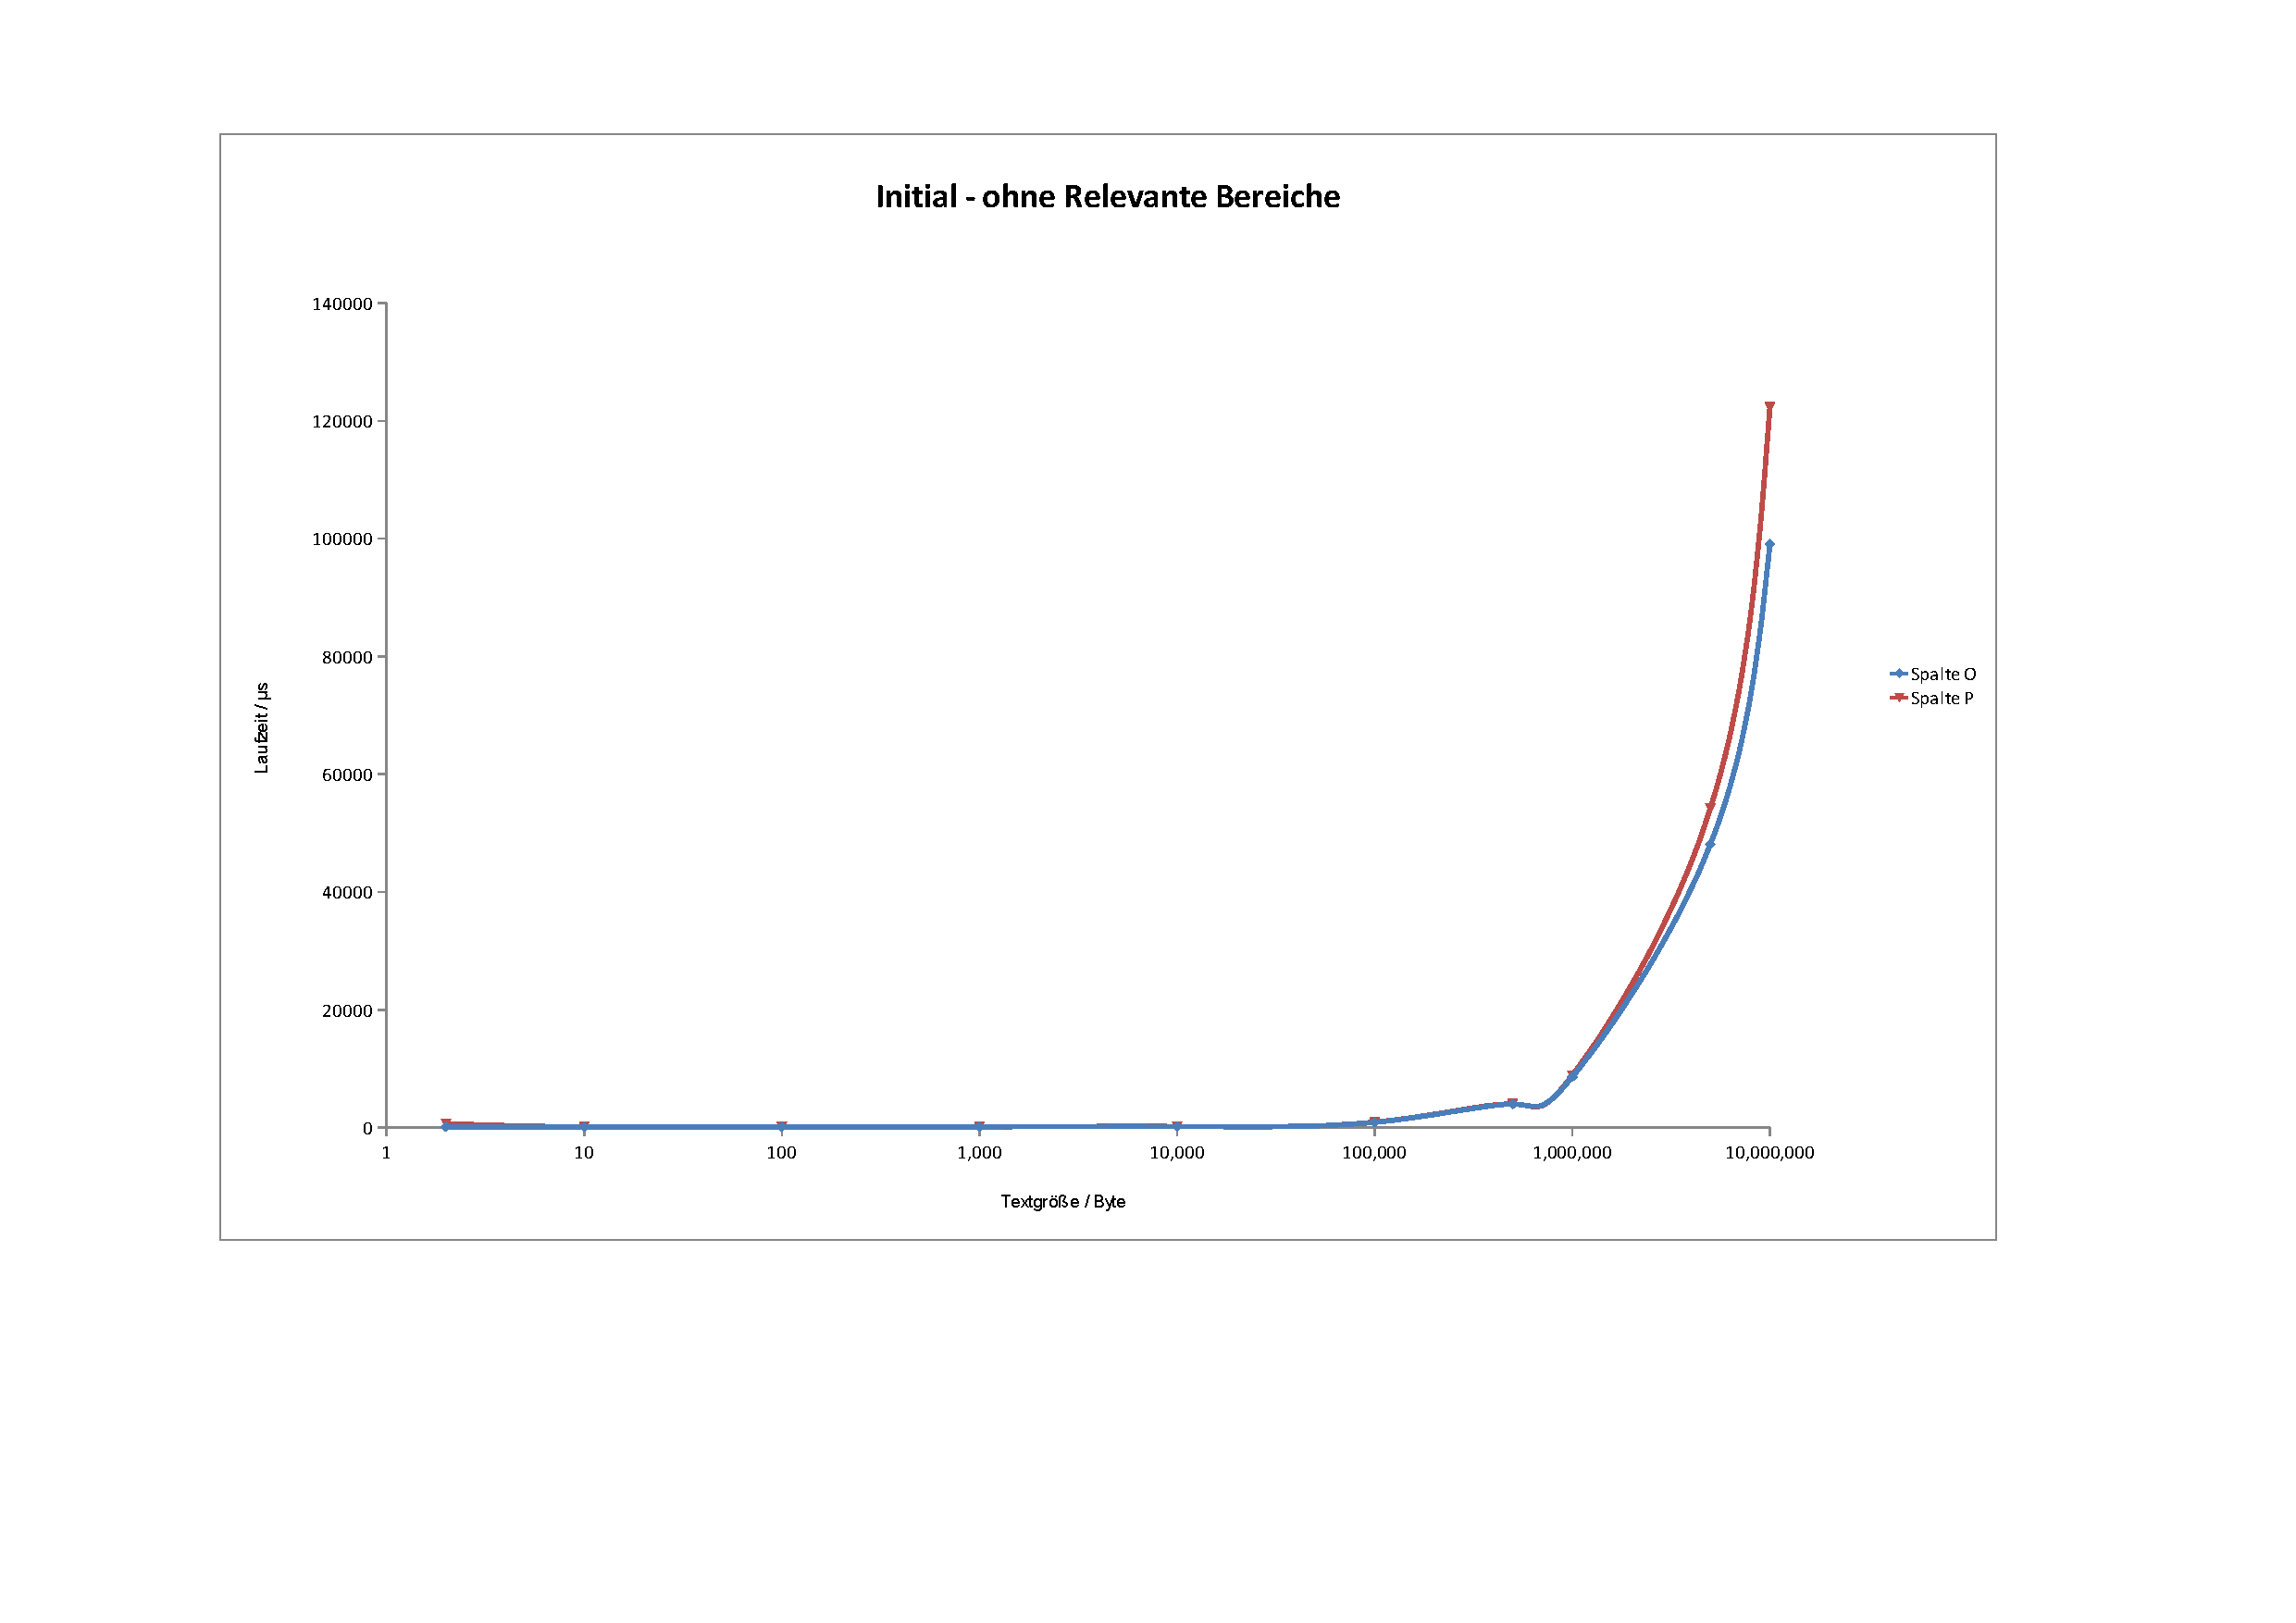
\includegraphics[width=\textwidth]{DiagrammInitial_worp.pdf}
	\label{fig:diagrammInitial_worp}
	\caption{Messung-Initial ohne relevante Bereiche}
\end{figure}

Der Nachteil gegenüber der Quellcodegrößen-Optimierung liegt jedoch darin, dass
mehr Speicherplatz in Anspruch genommen wird. Die Wahl der jeweiligen
Optmierungsmöglichkeit ist Situationsabhängig. Auf dem Mars könnten nur wenig
Speicherressourden zur Verfügung stehen, wodurch eine
Geschwindigkeitsoptimierung schwierig wäre. Die gleichen Betrachtungen ergeben
sich auch für alle anderen Messreihen (Abbildung \ref{fig:diagrammInitial_wrp},
\ref{fig:diagrammNormal_worp}, \ref{fig:diagrammNormal_wrp}). 

In Abbildung \ref{fig:diagrammInitial_wrp} ist die Laufzeit bezüglich
verschiedener Anzahlen relevanter Bereiche dargestellt. Die Textgröße bleibt
dabei stetig bei $5.000.000$ Byte. Damit ist ein Vergleich der Werte mit den
durchschnittlichen Werten der gleichen Textgröße aus Abbildung
\ref{fig:diagrammInitial_worp} möglich. Für nur wenige relevante Bereiche
unterscheiden sich die Werte maginal. Steigt die Anzahl, nimmt die Laufzeit
jedoch exponential zu (siehe Abbildung \ref{fig:diagrammInitial}) und Bewegen
sich im Millisekunden-Bereich. Das heißt, dass bei Verwendung einer sehr große
Anzahl an relevanten Bereichen das Protokoll an seine Grenzen stößt
(\todo{komisch ausgedrueckt iwi aber komm gerade auf nix anderes}).

\begin{figure}[H]
	\centering
	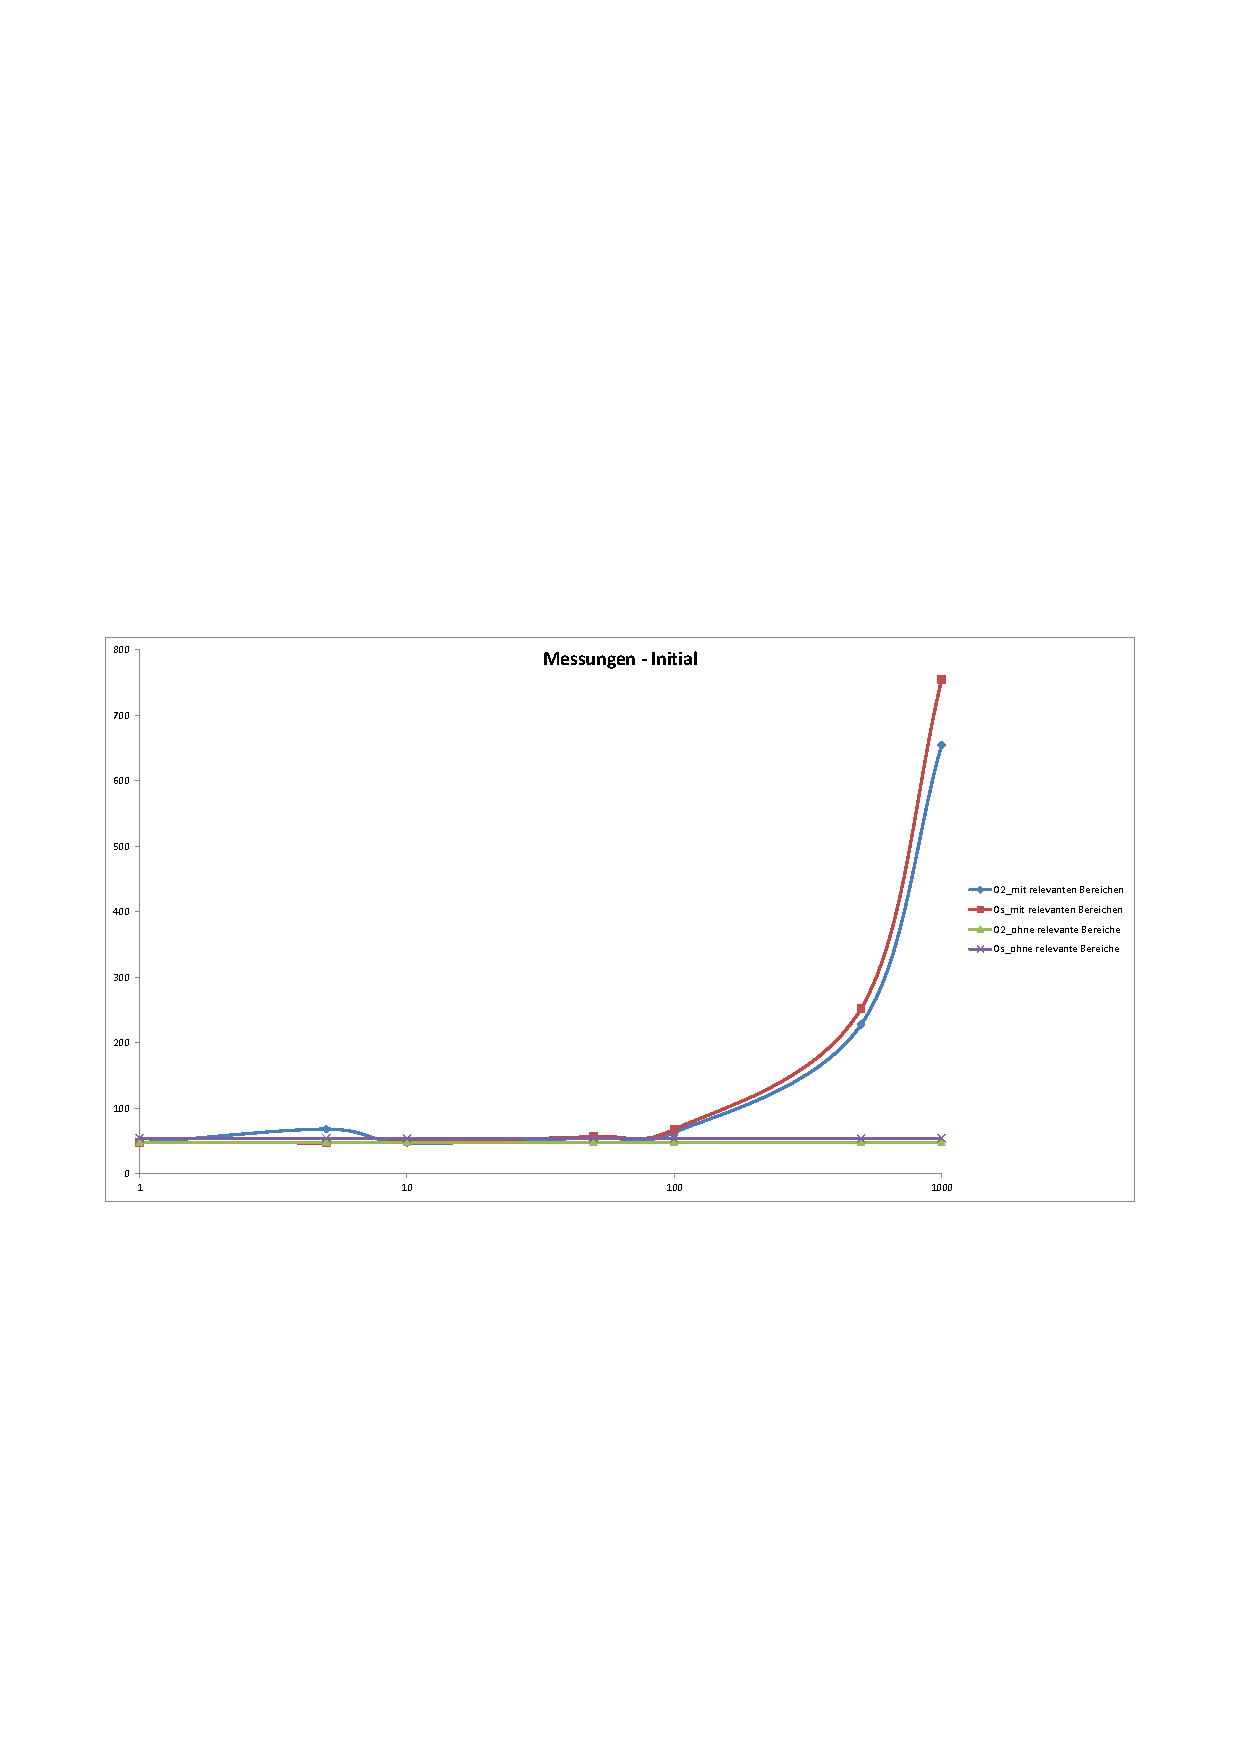
\includegraphics[width=\textwidth]{DiagrammInitial.pdf}
	\label{fig:diagrammInitial}
	\caption{Messung-Initial}
\end{figure}

\todo{fehlt noch der vergleich mit inital und normal \ldots aber weiß noch
nicht genau wie das aussehen soll. werden aber wahrscheinlich auch nur noch ein
paar sätze \ldots red ich mit flo jetzt nochmal drüber!}
